%% The following is a directive for TeXShop to indicate the main file
%%!TEX root = diss.tex

\chapter{Introduction}
\label{ch:Introduction}

Modern computer systems suffer from a huge speed gap between microprocessors and DRAM main memories. The traditional approach to tolerate the huge DRAM latency is to use huge multi-megabyte caches. However, caches often present us with a design tradeoff. While increasing cache size can lead to lower miss rates and thus better performance, it also requires higher silicon area, higher access latencies and consumes more power\cite{skadron1999branch}. In modern microprocessors caches often occupy a significant portion of the die area, and contribute to significant power consumption\cite{skylake,power9}. Figure \ref{fig:CacheSize} shows how area, dynamic energy, leakage power, and access latency scales with cache size. The results in Figure \ref{fig:CacheSize} were generated using CACTI\cite{cacti}.\par
\begin{figure}
    \begin{subfigure}[b]{0.5\textwidth}
        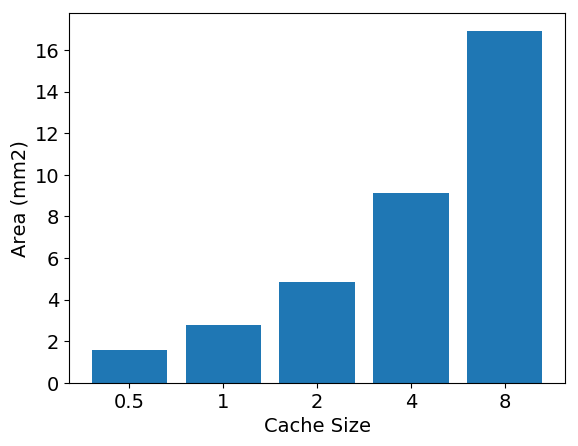
\includegraphics[width=\textwidth]{CacheArea.png}
        \caption{Cache Area vs. Cache Size}
    \end{subfigure}
    \begin{subfigure}[b]{0.5\textwidth}
        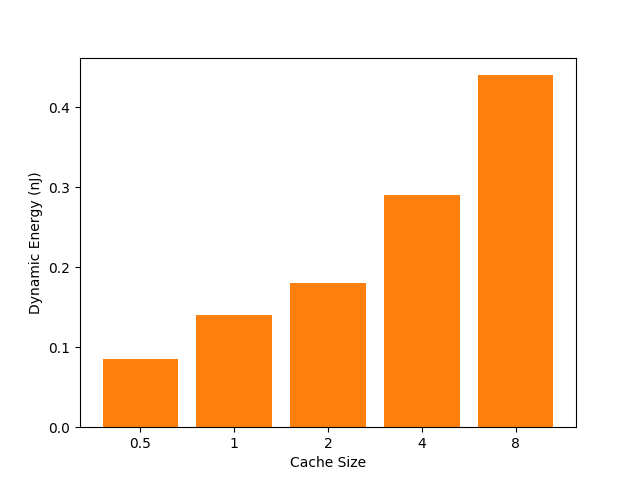
\includegraphics[width=\textwidth]{CacheEnergy.png}
        \caption{Dynamic Area vs. Cache Size}
    \end{subfigure}
    \begin{subfigure}[b]{0.5\textwidth}
        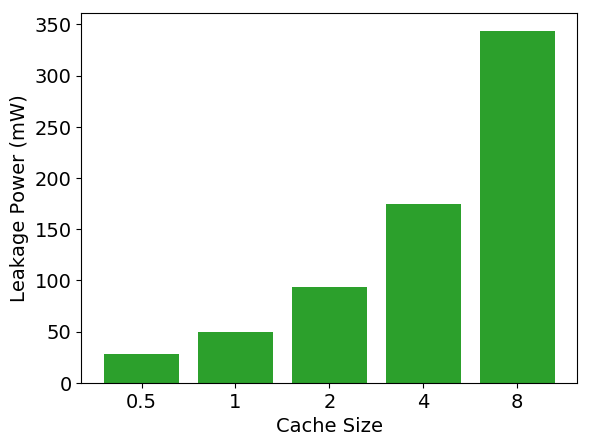
\includegraphics[width=\textwidth]{CachePower.png}
        \caption{Leakage Power vs. Cache Size}
    \end{subfigure}
    \begin{subfigure}[b]{0.5\textwidth}
        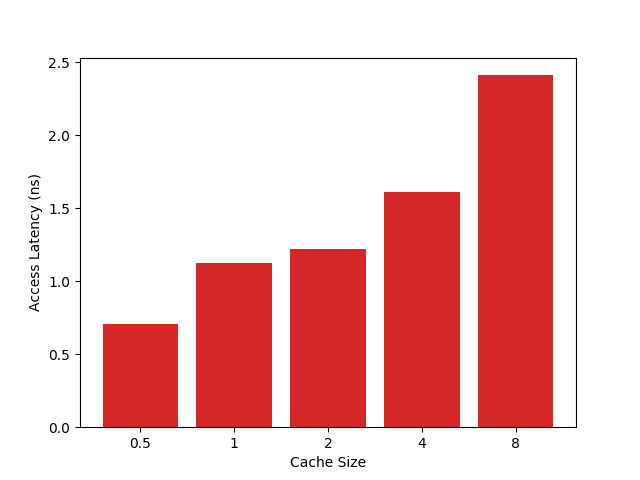
\includegraphics[width=\textwidth]{CacheLatency.png}
        \caption{Access Latency vs. Cache Size}
    \end{subfigure}
    \caption{Showing how different cache traits are affected by cache size.}
    \label{fig:CacheSize}
\end{figure}
A different approach that has gained more popularity recently is to use compression to better utilize the existing cache space instead of increasing cache sizes. Cache compression allows caches to store more than their physical sizes, essentially acting like bigger size caches. However, they also impose more constraints on the compression and decompression design, requiring it to be very fast to not affect the cache performance. Previous proposals discussed and exploited data similarities and redundancies on different granularities. Some studies have found that applications can exhibit a lot of zero cache lines, some proposals were completely focused on zero compression\cite{zca} while others treated zero lines as a special case in their compression schemes\cite{fpc, hycomp, dedup}. Other proposals took advantage of the existence of data similarities of different granularities across caches. Such approaches used dictionaries for intra-line granularity\cite{cpack, dish} or used deduplications\cite{dedup} to take advantage of inter-line granularity similarities. Some studies opted to do data compression to decrease the data size on a line or smaller granularity rather than exploit existing cache wide data patterns\cite{bdi, sc2, hycomp}.\par
The previously mentioned compression approaches do improve the utilization of cache space. However, each of those approaches focused on only one of two granularities to do compression. This first granularity was intra-line, only concerned about compressing data inside one data line to make the data line smaller and thus fit more than one data line in one physical cache line. The second granularity was inter-line, focusing only on reducing the total number of cache lines by getting rid of zero lines or deduplicating similar lines.\par
Some of today's applications can benefit from only one of those while others can benefit from both of them. For example, the dedup\cite{parsec} benchmark is only inter-line compressible through deduplication\cite{dedup}, the inversek2j\cite{axbench} benchmark is only intra-line compressible, while the bwaves\cite{spec} benchmark is compressible using both. It's obvious that only using one of the compressions on only one of the granularities is always missing some opportunity. Combining inter and intra-line compressions is the only way to gain the maximum possible compression and the highest benefits. But doing so also means that the cache organization is more complex, requires redesigning replacement policies, and more overhead. To our knowledge, no previous proposals have considered a compressed cache doing inter and intra-line compression at the same time.\par
In this work we pick two cache compression algorithms to cover inter and intra-line. We discuss their cache structures, compression, replacement policies, and their effect on different applications in Chapter \ref{ch:BackgroundMotiv}. Then we describe how to combine both compression schemes in a cache in Chapter \ref{ch:Design}. In the same chapter we also describe the effects and constraints it imposes on cache organization and replacement policies, and establish a roofline model for evaluation. In Chapter \ref{ch:Results} we show the results of our implementation against the two selected algorithms, we also show how the performance of our cache varies with multiple design choices and parameters. Chapter \ref{ch:Related Work} describes related cache compression techniques other than the two we picked.